This section presents the use case notation considered in the paper along with the tool support and an example of a distance function.

\subsection{CLARET and LTS-BT}
CLARET \cite{dalton2017claret,dalton2018mbtagile} is a DSL and tool that allows the creation of use case specifications using natural language. It was designed to be used as a central artifact for both requirement engineering and and MBT practices. Its toolset works as a syntax checker for use cases description files and provides
visualization mechanisms for use case revision. Listing 1 presents a use case specification using CLARET.  

From the use case description in Listing 1, CLARET generates its equivalent Annotated Labeled Transition System (ALTS) model \cite{tretmans2008model} (Figure \ref{fig:alts}). Transition labels starting with \textit{[c]} indicate pre or post conditions, while the ones starting with \textit{[s]} and \textit{[e]} are regular and exception execution steps, respectively.

\begin{figure}[h!] 
\centering 
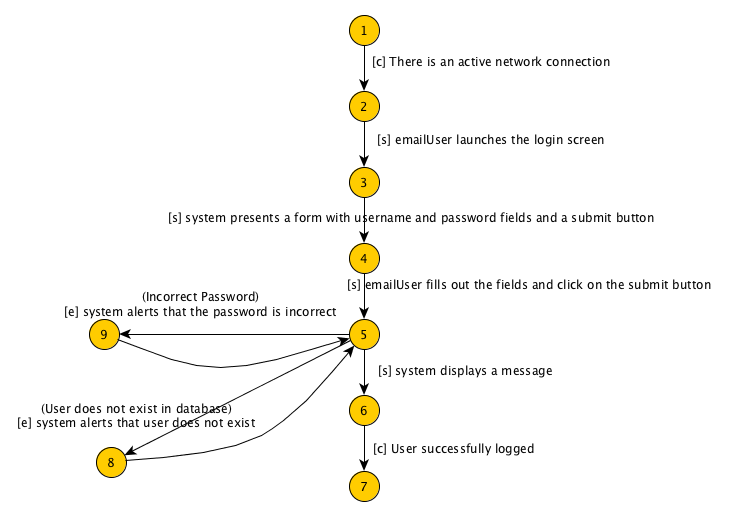
\includegraphics[width=.5\textwidth]{figs/UserLogin.png}
\caption{ALTS model of the use case from Listing \ref{specExample}.}
\label{fig:alts}
\end{figure}

CLARET's toolset includes a test generation tool, LTS-BT (Labeled Transition System-Based Testing) \cite{cartaxo2008lts}. LTS-BT is an MBT tool that uses as input LTS models and generates test suites by traversing them. The generated tests are reported in XML files that can be directly imported to a test management tool, TestLink\footnote{http://testlink.org/}. 
%Besides generation, it includes a series of algorithms for model-based test selection, reduction, and prioritization. 
The test cases reported in Section \ref{sec:motiv} were collected from running LTS-BT.

\subsection{Distance Functions}

Distance functions are metrics for evaluating how similar, or different, are two strings \cite{coutinho2016analysis}. Distance functions have been used in different contexts (e.g., \cite{runkler2000automatic,okuda1976method,lubis2018combination}). Moreover, there are several different distance functions (e.g., \cite{hamming1950error,han2007efficient:LCS,huang2008similaritycosine,de1mahalanobis:jaro,Levenshtein_SPD66}). For instance, the Levenshtein function \cite{Levenshtein_SPD66,kruskal1983overview} (equation described below) compares two strings (a and b) and calculates the number of required operations to transform a into b, and vice-versa; where $1_{ai \neq bj}$ is the indicator function equal to 0 when $a_{i} \neq b_{j}$ and equal to 1 otherwise, and $lev_{a,b}$ is the distance between the first $i$ characters of a and the first $j$ characters of b.

For instance, consider a = ``kitten'' and b = ``sitting'', the Levenshtein distance is three, since three operations are needed to transform a to b: (i) replacing `k' by `s'; (ii) replacing `e' by `i'; and (iii) inserting `g' at the end. 


\begin{equation*}
   lev_{a,b}(i,j) = 
    \begin{cases}
    max(i,j)  \qquad \qquad \qquad \qquad \qquad \text{if min(i,j) = 0}&\\
        min 
        \begin{cases}
            lev_{a,b}(i-1,j) + 1\\
            lev_{a,b}(i,j-1) + 1 & otherwise\\ 
            lev_{a,b}(i-1,j-1) + 1_{ai \neq bj} 
        \end{cases}
    \end{cases}
\end{equation*} 